% Created 2021-01-24 Sun 22:50
% Intended LaTeX compiler: pdflatex
\documentclass[11pt]{article}
\usepackage[utf8]{inputenc}
\usepackage[T1]{fontenc}
\usepackage{graphicx}
\usepackage{grffile}
\usepackage{longtable}
\usepackage{wrapfig}
\usepackage{rotating}
\usepackage[normalem]{ulem}
\usepackage{amsmath}
\usepackage{textcomp}
\usepackage{amssymb}
\usepackage{capt-of}
\usepackage{hyperref}
\usepackage{minted}
\hypersetup{colorlinks=true, linkcolor=black, filecolor=red, urlcolor=blue}
\usepackage[turkish]{babel}
\author{Eren Hatırnaz}
\date{10 Kasım 2019}
\title{Yazılım Gündemi - 17\\\medskip
\large 4-10 Kasım 2019}
\hypersetup{
 pdfauthor={Eren Hatırnaz},
 pdftitle={Yazılım Gündemi - 17},
 pdfkeywords={},
 pdfsubject={},
 pdfcreator={Emacs 27.1 (Org mode 9.3)},
 pdflang={Turkish}}
\begin{document}

\maketitle
\tableofcontents \clearpage\shorthandoff{=}

\begin{center}
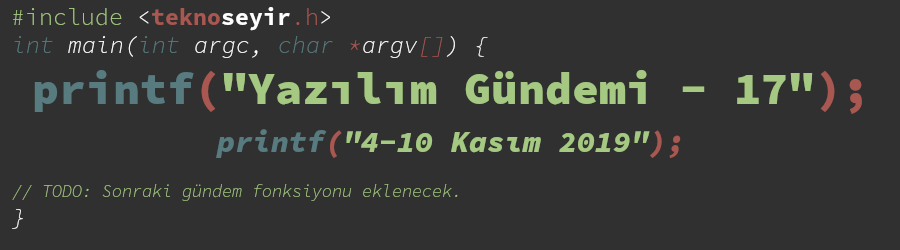
\includegraphics[width=.9\linewidth]{gorseller/yazilim-gundemi-banner.png}
\end{center}

\begin{center}
\href{../16/yazilim-gundemi-16.pdf}{< Önceki Gündem} | \textbf{4-10 Kasım 2019} | \href{../18/yazilim-gundemi-18.pdf}{Sonraki Gündem >}

\href{https://teknoseyir.com/blog/yazilim-gundemi-17-4-10-kasim-2019}{TeknoSeyir'de Oku}
\end{center}

\section{GitLab, önemli pozisyonlar için ülke \href{https://www.zdnet.com/article/gitlab-considers-ban-on-new-hires-in-china-and-russia-due-to-espionage-fears/}{kısıtlamasına gitmeyi tartışıyor}}
\label{sec:org7f6e76a}
\begin{center}

\includegraphics[height=3cm]{gorseller/gitlab-rusya-cin-engel.png}
\end{center}

Aslında tartışma yeni değil ilgili \href{https://gitlab.com/gitlab-com/www-gitlab-com/issues/5555}{issue sayfasında} da görülebileceği üzere
yaklaşık 3 hafta önce başlamış fakat yeni gündeme geliyor. Tartışmanın başlama
nedeni ise kurumsal müşterinin veri güvenliklerine ilişkin ilettiği kaygılar.
Bu doğrultuda GitLab da, Rusya ve Çin gibi ülkelerden şu iki pozisyon için
insan kabul etmeyecek: Site Güvenilirlik Mühendisi (Site Reliability Engineer)
ve Destek Mühendisi (Support Engineer). Ayrıca bu engelleme, güvenlik takımını
da etkiliyor. Bu iki pozisyondaki kişiler müşterilerin tüm verilerine
erişebiliyormuş. Bu nedenle, ilgili ülkelerdeki kişilerin bu rollerde olması
istenmiyor.

Çalışanların yaşadığı ülkelere göre izin sisteminin oluşturulması da ilgili
kişiler için bir "ikinci sınıf vatandaş" algısı oluşturup, kendilerini rahatsız
hissetmelerine yol açacağı için istenmiyor. Şimdilik en "insani" çözümün bu
olduğunu söyleyen GitLab yetkilisi, şu anda bu engelleme kabul edilirse bu
yolla hiçbir çalışanın etkilenmeyeceğini de belirtiyor.

Bu ülkelerden ilgili pozisyonlarda insan kaynağını alınmamasının yanı sıra eğer
bu konu kabul edilirse mevcut çalışanlar da bu listedeki ülkelere
taşınamayacaklar. Eğer taşınmak isterlerse işten ayrılmak zorunda kalacaklar.

Diğer açıdan bakacak olursak ismi geçen ülkelerin casusluk faaliyetleri de
sürekli gündemde olduğu için (hatta bu tartışma da yine Çin'in siber
ajanlarıyla ilgili bir \href{https://www.zdnet.com/article/building-chinas-comac-c919-airplane-involved-a-lot-of-hacking-report-says/}{raporun yayınlanmasından} sonra başladı) kurumsal
müşterilerin kaygıları da çok haksız sayılmaz. Üstelik bu engelleme yavaş yavaş
bir sektör pratiği haline de gelmeye başlamış. Maalesef kurunun yanında yaş da
yanıyor.

Bu hafta boyunca \href{https://news.ycombinator.com/item?id=21437334}{HackerNews} ve \href{https://www.reddit.com/r/gitlab/comments/dtfccm/gitlabs\_director\_of\_risk\_and\_global\_compliance/}{Reddit} gibi bir çok platformda tartışılan bu
konu elbette ilgili issue sayfasında da tartışılmaya devam etti. Bu tartışmalar
sırasında Candice Ciresi isimli GitLab'ın Global Risk ve Uyum Direktörü de aynı
issue içerisinde istifa ettiğini paylaştı fakat sonra bu yazı GitLab tarafından
kurallara uymadığı gerekçesiyle kaldırıldı. Yani bir nevi sansür uygulandı.
GitLab böyle bir davranış sergilemeseydi, "müşterilerinin kaygılarını gidermeye
çalışıyor" gözüyle bakmaya devam edecektim fakat böylesi sansürcü bir yaklaşımı
GitLab'a yakıştıramadım.

\begin{figure}[htbp]
\centering
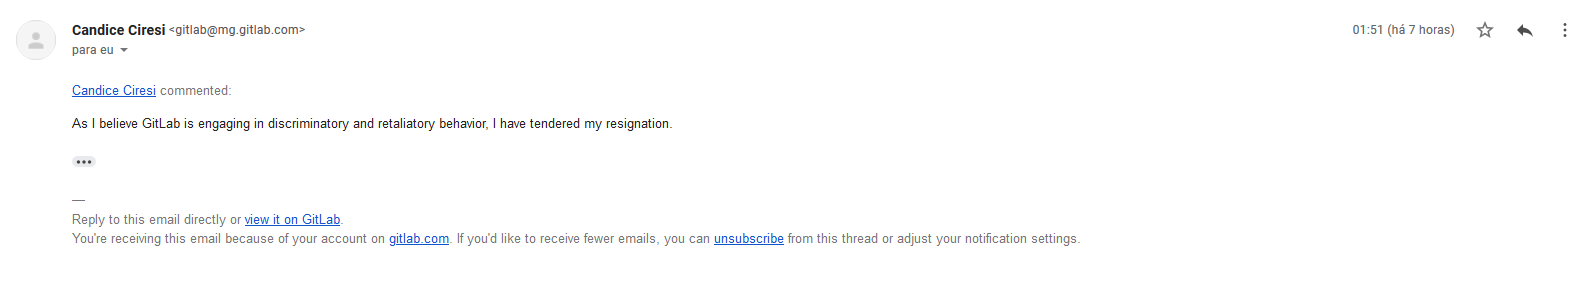
\includegraphics[width=.9\linewidth]{gorseller/gitlab-istifa-1.png}
\caption{Candice Ciresi'nin ilk gönderdiği mesaj (bir takipçiye giden mail)}
\end{figure}

\begin{figure}[htbp]
\centering
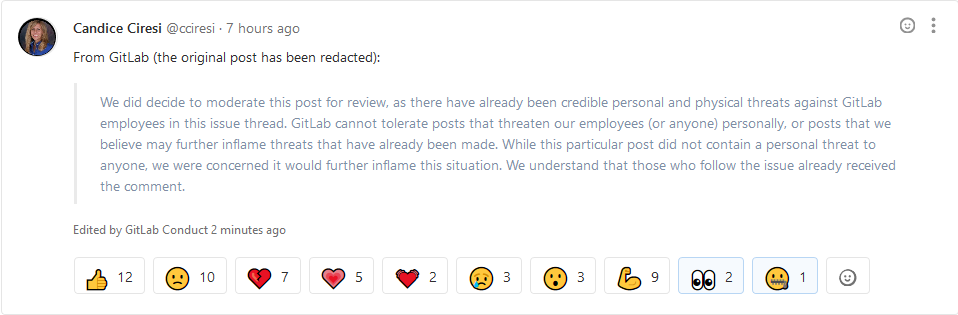
\includegraphics[width=.9\linewidth]{gorseller/gitlab-istifa-2.png}
\caption{GitLab'ın müdahalesi}
\end{figure}

Daha önceki yazılım gündemi yazılarından birinde de dediğim gibi, artık
internete bağlandığın konumun bir önemi olmadığı dönemler eskide kaldı (belki
de öyle bir dönem hiç olmadı, ambargo uygulanan bir ülkede olmadığımız için biz
fark edemedik), günümüzde maalesef hangi ülkeden internete çıktığın önemli
konulardan biri haline geldi.

Siz bu konuda ne düşünüyorsunuz? Böyle bir engelleme o ülkelerde yaşayan ya da
vatandaşı olan kişilere haksızlık mı, yoksa günümüz siber güvenlik çağında bir
mecburiyet mi? Yorumlar kısmında konuşalım.
\section{GitHub Sponsors özelliği \href{https://github.blog/2019-11-04-github-sponsors-is-now-out-of-beta-in-30-countries/}{30 ülkede betadan çıktı}}
\label{sec:org770d9c5}
Yaklaşık 6 ay önce GitHub, Sponsors özelliğini \href{https://techcrunch.com/2019/05/23/github-launches-sponsors-lets-you-pay-your-favorite-open-source-contributors/}{beta olarak duyurmuştu}. Bugün
ise yeni bir blog yazısı ile bu özelliğin 30 ülke için beta'dan çıktığını
duyurdular. Ülkelerin listesine \href{https://help.github.com/en/github/supporting-the-open-source-community-with-github-sponsors/becoming-a-sponsored-developer\#submitting-your-bank-and-tax-information}{bu adresten} bakabilirsiniz fakat sizi yormadan
ben söyleyeyim, Türkiye bu ülkeler arasında değil.

GitHub'ın yeni Sponsors özelliği için aslında bir nevi dahili Patreon sistemi
diyebiliriz. Aynı Patreon'da olduğu gibi kullanıcılar destek olmak istedikleri
projelere abonelik yöntemi ile 'sponsor' oluyorlar. Proje sahipleri isterlerse
farklı abonelik seviyeleri (ayda 1 dolar, ayda 5 dolar vb.) de oluşturabiliyor.

Eğer betadan çıkan 30 ülkenin birinde değilseniz, sizin ülkenize geldiğinde
haberdar olmak \href{https://github.com/sponsors}{bekleme listesine kayıt olup}, Beta programı için başvuru
yapabilirsiniz. GitHub, "resmi olarak varlık gösterdiğimiz diğer ülkelerde de
bu özelliği açmak için çalışıyor" diyor fakat Türkiye'de resmi olarak varlar
mı, bilgim yok ama umarım ülkemiz için de aktif olur.

Beta programındaki bazı proje sahipleri de şöyle bir \href{https://www.youtube.com/watch?v=7YcW25PHnAA}{kutlama videosu çekmişler}.

Güzel bir özellik, umarım açık kaynak ve özgür yazılım topluluğunun gelişmesine
vesile olur.
\section{GitHub yıllık \href{https://octoverse.github.com/}{Octoverse raporunu yayınlandı}}
\label{sec:org836ccdf}
GitHub, her yıl olduğu gibi bu yıl da GitHub'da 1 yıl boyunca olan bitenleri
rapor haline getirdi ve yayınlandı. Bu hafta \href{https://github.blog/2019-11-06-the-state-of-the-octoverse-2019/}{bir blog yazısı} yazarak yeni
Octoverse raporlarını duyurdular. Şimdi isterseniz rapordan birkaç başlığı
birlikte inceleyelim:

\subsection{Topluluk}
\label{sec:orga3f14e2}
2019 yılı boyunca:
\begin{itemize}
\item GitHub'a toplam 10 milyon yeni kullanıcı katılmış ve toplam da 40 milyon
üzeri kullanıcı sayısına çıkılmış.
\item 44 milyon yeni depo yaratıldı ya da "fork" edildi ve 2018'e göre \%44 daha
fazla geliştirici ilk deposunu yarattı
\item 87 milyon pull request kabul edilmiş ve 2018'e göre \%28 daha fazla
geliştirici ilk pull request'ini oluşturmuş.
\item 20 milyon issue kapatılmış.
\item 2.9 milyon organizasyon sayfası oluşturulmuş.
\end{itemize}
\subsection{Ülkeler}
\label{sec:org0f3752d}
\begin{figure}[htbp]
\centering
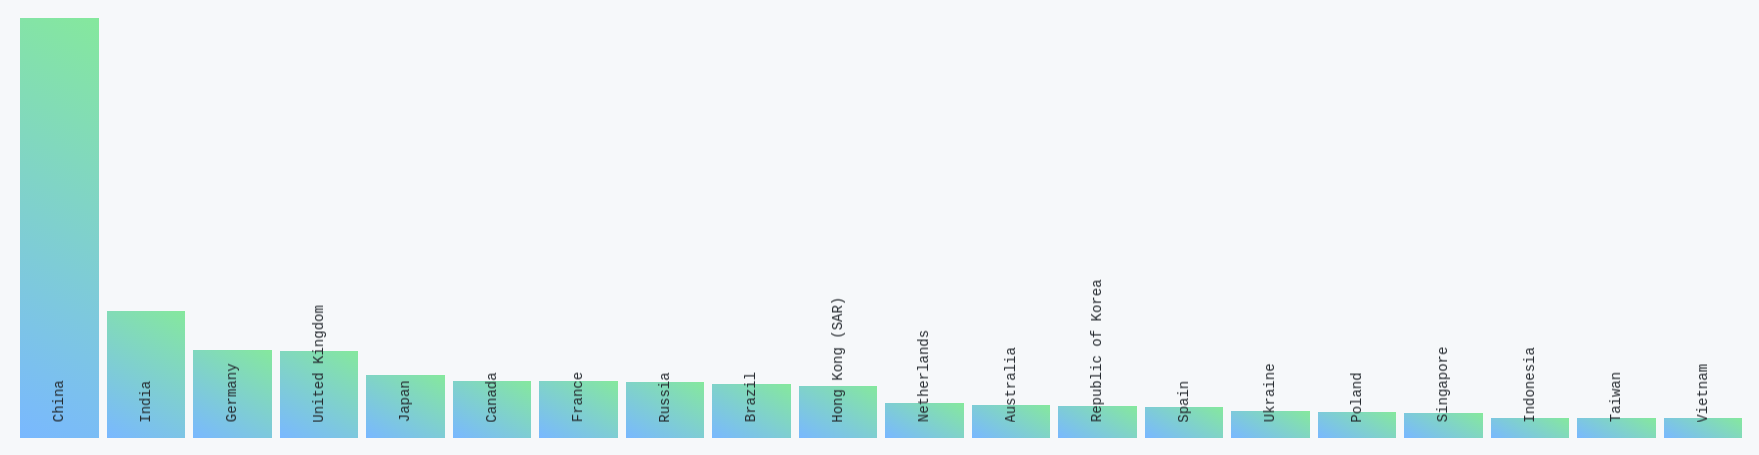
\includegraphics[width=.9\linewidth]{gorseller/github-ulke-kullanim.png}
\caption{En çok açık kaynak kullanan (fork ve clone sayısına göre) ülkeler}
\end{figure}

\begin{figure}[htbp]
\centering
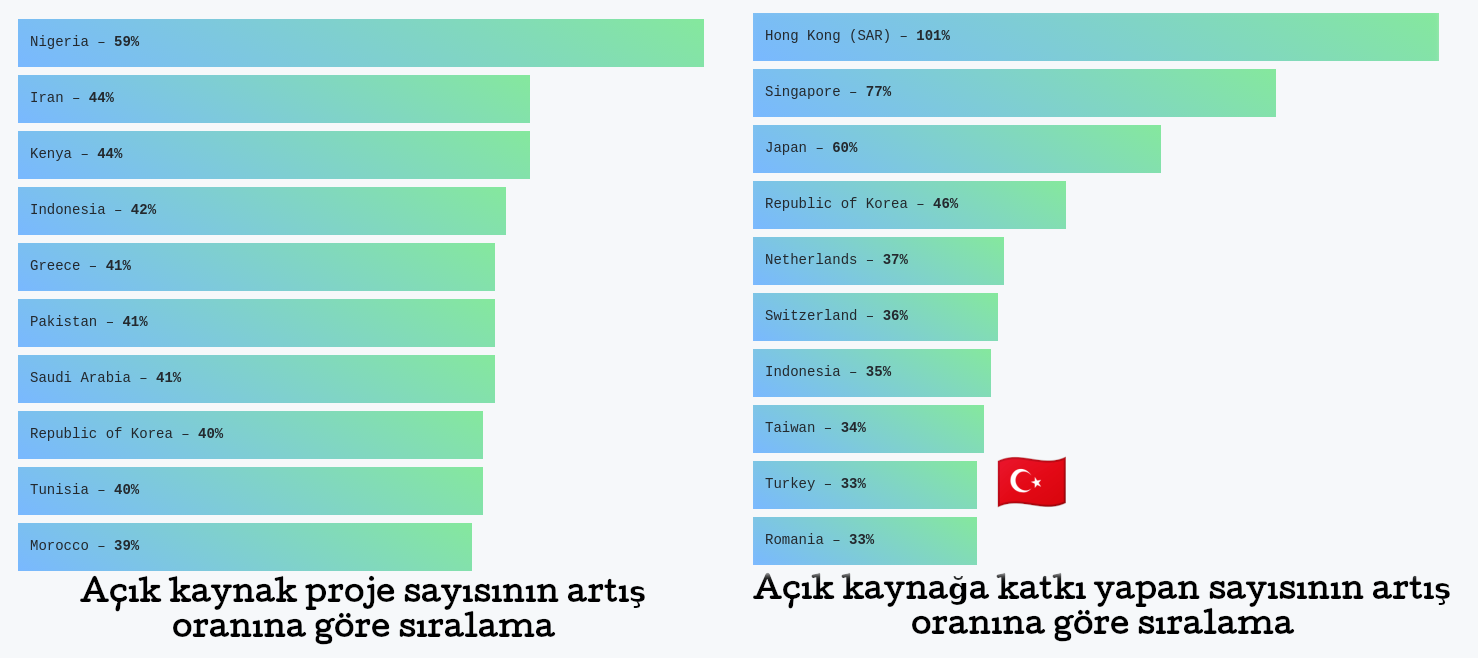
\includegraphics[width=.9\linewidth]{gorseller/github-ulkeler-acik-kaynak.png}
\caption[\textbf{(SOL):} \textbf{(SAĞ):}]{\textbf{(SOL):} Açık kaynak proje sayısının artış oranına göre sıralama \textbf{(SAĞ):} Açık kaynak katkı yapan sayısının artış oranına göre sıralama}
\end{figure}

Açıkcası bu sıralama beni şaşırttı çünkü önceki yazılım gündemi yazılarından
hatırlayacağınız üzere GitHub, Amerika'nın yaptırımlarını uygulamaya başlamış
ve İran'lı geliştiricilerin hesaplarına bazı kısıtlamalar getirmişti (bkz:
\href{../03/yazilim-gundemi-03.pdf}{Yazılım Gündemi - 3}). Buna rağmen İran'ın bu listede ikinci sırada yer alması
şaşırtı beni. Gerçi bu olay Temmuz ayında gerçekleşti ama demek ki bu olaydan
önce yaratılan açık kaynak depolar bile \%44 oranını sağlamış.

Sağdaki sıralama da beni bir o kadar şaşırttı. Ne yalan söyleyeyim listede
Türkiye'yi görmeyi beklemiyordum. Diğer ülkelere göre alt sıralarda olsak da,
açık kaynağa katkı yapanlar sayısındaki artış sevinmeme yetiyor. Umarım
ilerleyen yıllarda daha da artar.
\subsection{Programlama Dilleri}
\label{sec:org2b93b05}
\begin{figure}[htbp]
\centering
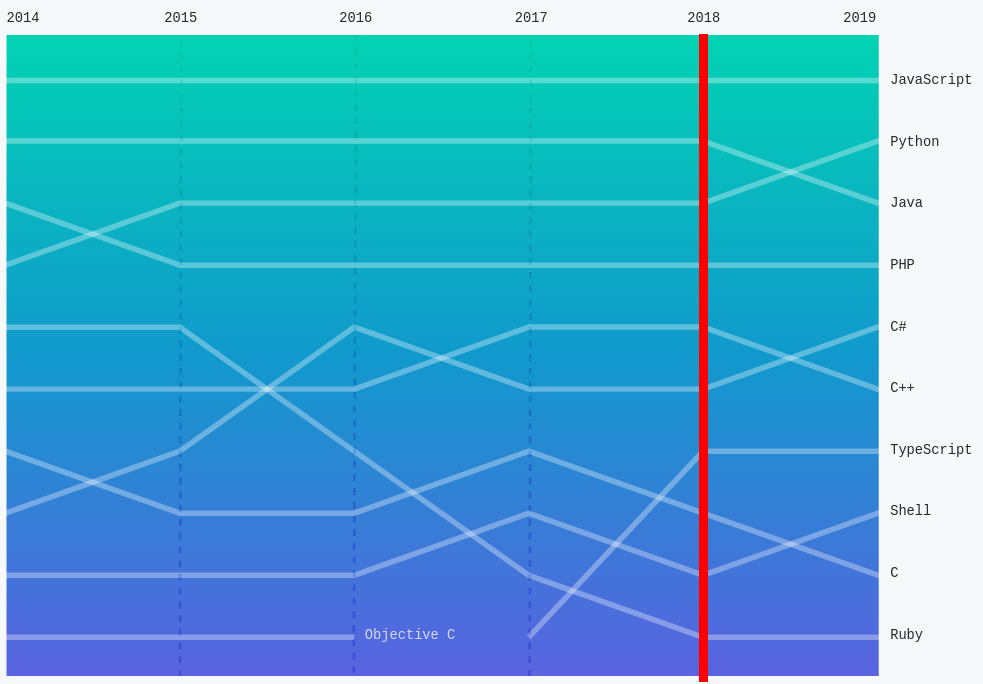
\includegraphics[width=.9\linewidth]{gorseller/github-populer-diller.png}
\caption{Popüler ilk 10 programlama dili sıralaması}
\end{figure}

Gelelim popüler ilk 10 programlama dilleri sıralamasına. JavaScript 2014'den
beri gelen liderliğini koruyor fakat Java, "İkinci en popüler programlama
dili" unvanını Python'a kaptırıyor. PHP ise dördüncülük unvanını kimseye
bırakmıyor. Listenin devamında ise C\# ve C++ arasındaki çekişmeli mücadeleyi
görmekteyiz. Ardından geçtiğimiz senelerde ilk 10'a girmeyi başaran
TypeScript'in yerini koruduğunu görürken; Shell ve C arasında bir değiş tokuş
gerçekleştiğini gözüküyor ve son olarak zaman içerisinde popülaritesinin
düşüşüyle beni şaşırtan Ruby dilini onuncu sırada görmekteyiz.

Burada şu uyarısı yapmadan geçemeyeceğim: Bu listelerin projenize uygun dili
seçme aşamasında sizi etkilemesine izin vermeyin. Sonuçta programlama dilleri
birer araç ve biz de yapacağımız işe en uygun aracı seçip onu kullanıyoruz.
Sırf popüler diye bir programlama dilini seçmek ileride teknik anlamda sizi
zora sokabilir.
\section{Microsoft, \href{https://visualstudio.microsoft.com/services/visual-studio-online/}{Visual Studio Online} hizmetini duyurdu}
\label{sec:org484a768}
Yaklaşık birkaç senedir uzaktan kod yazmaya olanak sağlayan hizmet ve
araçların sayısındaki yükseliş gözüme çarpıyordu ki Microsoft da bu alanda bir
şeyler görmüş olacak ki Visual Studio Code yazılımını, Visual Studio Online
olarak uzaktan tarayıcı üzerinden çalışacak hale getirmiş ve Azure
ekosistemine yeni bir parça daha eklemiş.

Denemek için \href{https://online.visualstudio.com}{online.visualstudio.com} adresinden bir geliştirme ortamı
oluşturmaya çalıştım fakat aktif bir Azure aboneliği istiyor. 1 aylık bedava
Azure aktifleştirmeye çalıştım fakat o da kredi kartı bilgileri isteyince
vazgeçtim. Aslında bu yıl içerisinde yayınlanmış ve sonradan \href{https://coder.com}{coder.com} isminde
bir girişime dönüşmüş, şu açık kaynak çözüm de sanırım fikir vermesi açısından
denenebilir: \url{https://github.com/cdr/code-server}. Sonuçta Microsoft'un kendisi
de yine VS Code yazılımının alt yapısını kullanarak bu hizmeti oluşturdu.
Yalnız şöyle bir şey var, ben Firefox ile açmaya çalıştığımda çok kısa bir
"tarayıcınız şimdilik desteklenmiyor" deyip hemen ana sayfaya yönlendirdi.
Chrome ile deneyince açıldı. İlginç\ldots{}

Yalnız bu yeni hizmetin ismi konusunda biraz kafam karışık. Microsoft'un zaten
Visual Studio Online isminde bir GitHub ve GitLab benzeri kod barındırma
hizmeti sunduğu bir servisi vardı. [kullanıcı\_adın].visualstudio.com şeklinde
bir alan adresi veriyordu ve orada aynı GitHub gibi kodlarınızı barındırıp,
issue açıp, proje yönetebiliyordunuz. Hatta ben 2013 yılında birtakım
projelerim için kullanıyordum fakat görünen o ki Microsoft, bu isimi daha çok
uygun olan bir projeye aktarmış. Benim kullandığım hizmetin ismi de Azure
DevOps olmuş sanırım. Gerçi emin de değilim uzun zamandır Microsoft
teknolojilerinden uzak olduğum için bu isim değişikliğinden haberim olmamış da
olabilir.

Bu konu hakkında siz ne düşünüyorsunuz? Bu şekilde geliştirme ortamınızı buluta
taşımak ister misiniz, yoksa "yok arkadaş ben kendi bilgisayarımda tutarım her
şeyimi" diyenlerden misiniz? Ben şahsen ikincisiyim. Belki biraz geri kafalılık
da sayılabilir bilmiyorum ama tarayıcı üzerinden kod yazmak bana biraz garip
geliyor. Ayrıca Levent Abi'nin söylemini tekrar hatırlatmakta fayda var: "Bulut
dediğin başkasının bilgisayarıdır. Bir gün gelir de, 'sana hizmet vermiyorum'
derse kalırsın öyle ortada" (bkz: \href{../03/yazilim-gundemi-03.pdf}{Yazılım Gündemi - 3}). Bu doğrultuda
endişelerimin de haklı olduğunu düşünüyorum.
\section{Git 2.24 \href{https://raw.githubusercontent.com/git/git/master/Documentation/RelNotes/2.24.0.txt}{sürümü duyuruldu}}
\label{sec:orga85495d}
Artık versiyon kontrol sistemlerinin lideri haline gelen Git, bu hafta
içerisinde 2.24 numaralı sürümünü duyurdu. Birkaç değişikliği birlikte
inceleyelim:

\subsection{Yeni özellik makroları}
\label{sec:orge2b0012}
Git çok uzun zamandır hem global hem de sadece depo bazında ayarlar yapmamıza
izin veren \texttt{git config} ile kullandığımız ayar alt sistemine sahip. Hem
kendinizi tanıtmak için hem de bazı özellikleri açıp kapatabilmek ya da
özelleştirmeler yapabilmek için \texttt{.gitconfig} isimli dosyası komut yardımıyla
ya da elle düzenlememiz gerekiyor. Fakat bazen yeni gelen bazı özellikleri
keşfetmek ve ayar yapmak bazen fazla zaman alıcı olabiliyor. Bu yüzden artık
Git geliştiricileri bazı yeni özellikler için makro sistemi geliştirler ve
şöyle bir komut ile özellikleri açıp kapatabileceğiz:
\begin{verbatim}
$ git config feature.manyFiles true
\end{verbatim}
Bu komutu çalıştırdığınızda Git sizin için o özellikle ilgili ayarları
düzenliyor. Bu makrolar Git geliştiricileri tarafından önceden belirlenmiş
olarak geliyor.
\subsection{Tarihçeyi yeniden yazmak için alternatif araçlar}
\label{sec:org96143ca}
Projelerde çalışırken, her ne kadar yapılması tavsiye edilmese de bazen
belirli nedenler ötürü Git tarihçesini yeniden yazmamız gerekebiliyor. Mesela
bir dosyayı tüm commit'lerden silmek gibi. Şimdiye kadar bunun için \texttt{git
	 filter-branch} aracı kullanıyorduk, fakat bu aracın kullanımı biraz karışık
olabiliyordu. Bu nedenle Git geliştiricileri yeni bir araç geliştirdiler: \texttt{git
	 filter-repo}. Bu araç ile:
\begin{itemize}
\item \texttt{git filter-repo -{}-analyze} komutu ile artık depomuz hakkındaki bazı
ölçümlerle ilgili bilgiler alabileceğiz. Mesela kaç tane obje olduğu, en
büyük dosyaların ya da klasörlerin hangileri olduğu gibi. Bunun gibi
bilgiler veren başka bir araça göz atmak isterseniz: \href{https://github.com/github/git-sizer}{git-sizer}
\item \texttt{-{}-path-\{glob-regex\}} ile artık tarihçeyi sadece belirli bir dizin için
değiştirken glob ve regex kullanabileceğiz.
\item Diğerine göre daha genişletilebilir bir araç olduğu için artık kendimiz
bazı alt komutlar ekleyebileceğiz. Demo için şu adresdeki depoya göz
atabilirsiniz: \href{https://github.com/newren/git-filter-repo/tree/master/contrib/filter-repo-demos}{newren/git-filter-repo}
\end{itemize}

Diğer özellikler ve yenilikler için GitHub'ın yayınladığı \href{https://github.blog/2019-11-03-highlights-from-git-2-24/}{bu blog yazısı} çok
faydalı olabilir. Ben de bundan faydalandım.
\section{Google, Android 11'de AsyncTask API'sini \href{https://www.xda-developers.com/asynctask-deprecate-android-11/}{kaldırmaya hazırlanır}}
\label{sec:orgce2aec2}
Asenktron işler, programlamanın hemen her alanında işimize çok yarayan ve
gerekli olan yapılar. Çünkü bir web sunucusundan veri çekerken kullanıcıların
ekranlarını dondurmak istemeyiz. Android tarafında da bu tarz asenkron işler
için Google tarafından sisteme eklenmiş bir API var. Android geliştirmede pek
deneyimim olmasa da xda-developers sitesindeki yazıdan anladığım kadarıyla bu
API biraz sorunluymuş. Şöyle ki bazı durumlarda asenkron iş tamamlandığında
uygulamanın ilgili görsel tarafı artık var olmayabilir (kullanıcı başka bir
ekrana geçmiştir vs.) fakat AsyncTask API'si bunu kontrol etmediği için
uygulamanın çökmesine yol açabiliyor. Elbette siz manuel olarak bazı kontroller
ekleyebilirsiniz ama bu sefer de kod tekrarı gibi şeyler oluşabiliyor. Bu gibi
nedenlerden dolayı Google da, sanırım fazla da kullanılmayan bir API olduğu
için, \href{https://android-review.googlesource.com/c/platform/frameworks/base/+/1156409}{bunu deprecate etmeye karar verdi}. Bu ifadeyi Türkçe'ye tam nasıl
çeviririz bilemiyorum ama biraz açmak gerekirse: API tam olarak kaldırılmayacak
ama artık desteklenmeyecek ve kullanılması da tavsiye edilmeyecek. Zaten
xda-developers sitesindeki yazıdan anladığım kadarıyla pek tercih edilen de bir
API değilmiş. Android geliştirici arkadaşlar da doğrulayabilirler sanırım. Çoğu
geliştirici onun yerine daha esnek \href{https://github.com/ReactiveX/RxJava}{RxJava} ya da Kotlin tarafında \href{https://kotlinlang.org/docs/reference/coroutines-overview.html}{Coroutines}
kütüphanelerini kullanıyor.

Android geliştiricisi arkadaşlar için pek büyük bir kayıp sayılmasa da
kullanan arkadaşlar varsa artık yeni kütüphanelere geçmelerini tavsiye ederim.
\section{Gradle 6.0.0 \href{https://docs.gradle.org/6.0/release-notes.html}{yayınlandı}}
\label{sec:org947f2ea}
Yazılım geliştirme süreçlerinin evrildiği hal itibariyle artık 3. parti
kütüphaneler olmadan çözümler geliştirmek pek mümkün gözükmüyor. Haliyle biz
de bu 3. parti kütüphaneleri ve derleme işlemlerini yönetmek için araçlara
ihtiyaç duyduk. İşte \href{https://gradle.org/}{Gradle} da bu araçlardan birisi. Her ne kadar C++ ve
JavaScript gibi dillerde desteği olsa da daha çok Java ekosisteminde ve
Android uygulama geliştirme alanlarında daha çok tercih edilen bir araç. Bu
hafta itibariyle de 6.0.0 sürümünü duyurdu. Bu sürümde duyurulan bir
değişikliği birlikte inceleyelim:

\subsection{Java ve Groovy için daha hızlı derleme}
\label{sec:orgb332e88}
Direkt bir örnekle açıklamak gerekirse:
\begin{minted}[breaklines=true,breakanywhere=true,frame=lines, linenos, label=Java, labelposition=topline]{java}
class A {}

class B {
    static void foo() {
        A a1 = new A();
    }
}

class C {
    void bar() {
        B.foo();
    }
}
\end{minted}
Buradaki her sınıfı ayrı bir dosya olarak düşünün. Gradle'ın önceki
sürümlerinde \textbf{A} sınıfında bir değişiklik olduğunda tüm diğer dosyalar da
yeniden derleniyordu fakat artık sadece \textbf{A} ve \textbf{B} sınıfları derlenecek.
Çünkü \textbf{A} sınıfın değişmesi \textbf{C} sınıfını doğrudan ilgilenmiyor. O sadece \textbf{B}
sınıfındaki bir fonksiyonu çağırıyor. Böylece derlenecek dosya sayısındaki
azaltma da derleme hızlarını olumlu olarak etkiliyor.

Diğer özellik ve değişiklikler için konu başlığına eklediğim bağlantıya
tıklayabilirsiniz.
\section{Visual Studio Code \href{https://code.visualstudio.com/updates/v1\_40}{Ekim 2019 sürümü duyuruldu}}
\label{sec:orgbe7fc2e}
\begin{center}
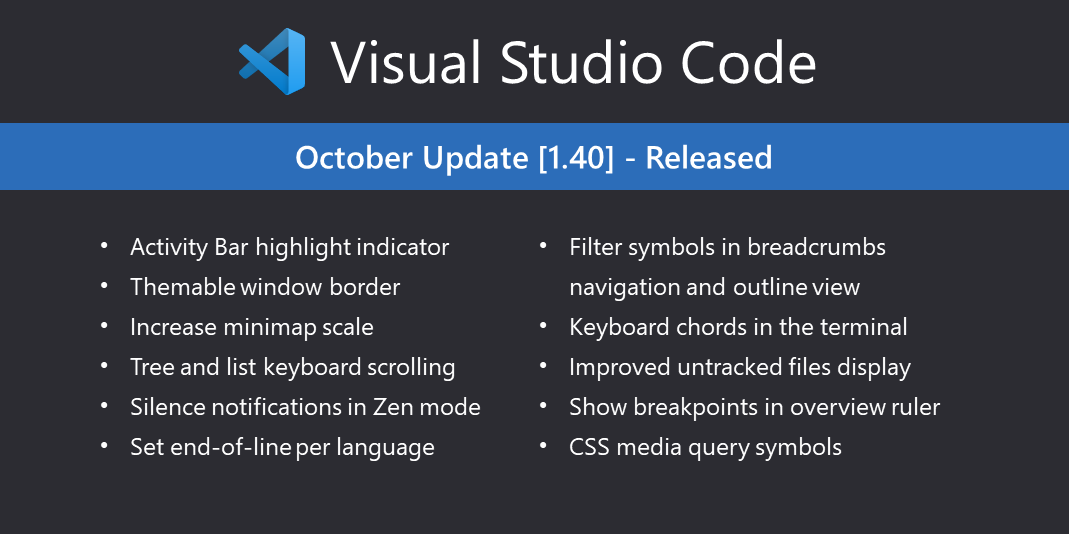
\includegraphics[width=.9\linewidth]{gorseller/vscode1-40.png}
\end{center}
\section{Anket: \href{https://docs.google.com/forms/d/e/1FAIpQLScDKFrhI4SeTuRtokSNYrdSrNKdM8zmHkPyNfMxIG3PgXnQNg/viewform}{Türkiye Açık Kaynak Platformu Talep Analizi Anketi}}
\label{sec:org9a54700}
Türkiye Açık Kaynak platformu çalışmaları devam ediyor. Konu başlığına
eklediğim ankete katılarak fikir ve önerilerinizi paylaşabilirsiniz. Türkiye
Açık Kaynak Platformu hakkında ümitliyim, umarım yakın zamanda bir şeyler
ortaya çıkar.
\section{Yaklaşan Etkinlikler}
\label{sec:org11c9cba}
\begin{longtable}{|p{8cm}|l|l|}
\hline
Etkinlik İsmi & Yeri & Tarihi\\
\hline
\endfirsthead
\multicolumn{3}{l}{Önceki sayfadan devam ediyor} \\
\hline

Etkinlik İsmi & Yeri & Tarihi \\

\hline
\endhead
\hline\multicolumn{3}{r}{Devamı sonraki sayfada} \\
\endfoot
\endlastfoot
\hline
\href{https://www.eventbrite.com/e/2020-ve-sonras-icin-yazlm-test-trendleri-tickets-78599383873}{2020 ve Sonrası için Yazılım Test Trendleri} & Ankara & 14 Kasım 14:00\\
\href{https://kommunity.com/devnot-yazilimci-bulusmalari/events/flutter-ile-ilk-mobil-uygulamanizi-yazin}{Flutter ile İlk Mobil Uygulamanızı Yazın} & İstanbul & 15 Kasım 19:00\\
\href{https://www.eventbrite.com/e/cyber-security-summit-tickets-73829151981}{Cyber Security Summit} & İstanbul & 16 Kasım 09:00\\
\href{https://kommunity.com/tensorflow-turkey/events/tensorflow-world-extended-ankara}{TensorFlow World Extended Ankara} & Ankara & 16 Kasım 13:00\\
\hline
\end{longtable}
\section{Diğer Haberler}
\label{sec:org2b9d663}
\begin{itemize}
\item Bazı çalışanlar, Google'ın petrol şirketleri ile yaptığı \href{https://www.bloomberg.com/news/articles/2019-11-04/now-googlers-are-protesting-company-s-cloud-deals-with-big-oil}{iş anlaşmalarını
protesto etti}.
\item Electron bazlı uygulamalar Mac uygulama mağazasından \href{https://www.theregister.co.uk/2019/11/05/apple\_app\_store\_electron}{atılma tehdidi ile
karşı karşıya}. \href{https://onezero.medium.com/apple-is-trying-to-kill-web-technology-a274237c174d}{Blog yazısı}, \href{https://news.ycombinator.com/item?id=21486430}{HackerNews}, \href{https://www.reddit.com/r/programming/comments/dtuv4v/apple\_is\_trying\_to\_kill\_web\_technology}{Reddit}.
\item JetBrains, IntellijIdea için geliştirdiği yeni \href{https://blog.jetbrains.com/idea/2019/11/meet-grazie-the-ultimate-spelling-grammar-and-style-checker-for-intellij-idea/}{yazım denetimi aracını
tanıttı}: \href{https://plugins.jetbrains.com/plugin/12175-grazie/}{Grazie}.
\item Kendi sunucusunda GitHub çalıştıranlar için GitHub Actions \href{https://github.blog/2019-11-05-self-hosted-runners-for-github-actions-is-now-in-beta/}{beta olarak
duyuruldu}.
\item OpenAI organizasyonunun metin oluşturma yapay zekası \href{https://openai.com/blog/gpt-2-1-5b-release/}{GPT-2 yayınlandı}.
\href{https://www.theverge.com/2019/11/7/20953040/openai-text-generation-ai-gpt-2-full-model-release-1-5b-parameters}{Alternatif}
\item Google, Cardboard yazılımını \href{https://www.theverge.com/2019/11/6/20952495/google-cardboard-open-source-phone-based-vr-daydream}{açık kaynak yaptı}. \href{https://github.com/googlevr/cardboard}{GitHub Deposu}
\item Postman'den yeni görselleştirme \href{https://blog.getpostman.com/2019/11/04/visualizing-apis-of-the-world/}{aracını duyurdu}: \href{https://www.getpostman.com/api-visualizer}{API Visualizer}.
\item Microsoft SRC takımı, Windows içerisinde Rust kullanım alanları ile \href{https://msrc-blog.microsoft.com/2019/11/07/using-rust-in-windows/}{ilgili
bir blog yazısı paylaştı}.
\item WinUI 3.0 Alpha \href{https://github.com/microsoft/microsoft-ui-xaml/issues/1531}{duyuruldu}.
\item PHP topluluğu, Union Types özelliği önerisini \href{https://github.com/php/php-rfcs/pull/1\#issuecomment-551454495}{kabul etti}. \href{https://wiki.php.net/rfc/union\_types\_v2}{Öneri detayları
sayfası}
\item Go programlama dili \href{https://blog.golang.org/10years}{10 yaşında}.
\item TypeScript 3.7 final \href{https://devblogs.microsoft.com/typescript/announcing-typescript-3-7/}{sürümü yayınlandı}.
\item Rust programlama dilinin \href{https://blog.rust-lang.org/2019/11/07/Rust-1.39.0.html}{1.39.0 sürümü duyuruldu}.
özellikleri hakkında \href{https://blog.rust-lang.org/2019/11/07/Async-await-stable.html}{özel blog yazısı yayınlandı}.
\item D programlama dilinin \href{https://dlang.org/blog/2019/11/06/dmd-2-089-0-released/}{2.089.0 sürümü yayınlandı}.
\item Dart programlama dilinin \href{https://medium.com/dartlang/dart2native-a76c815e6baf}{2.6 sürümü yayınlandı}.
\item Facebook, sıkıştırma algoritması zstandard'ın \href{https://github.com/facebook/zstd/releases/tag/v1.4.4}{1.4.4 sürümünü duyurdu}.
\item KDAB, yeni bir Qt komponenti \href{https://www.kdab.com/kddockwidgets/}{duyurdu}: \href{https://github.com/KDAB/KDDockWidgets}{KDDockWidgets}.
\item Açık kaynak 3 boyutlu grafik motoru Ogre, \href{https://www.ogre3d.org/2019/11/05/ogre-1-12-3-released}{1.13.3 sürümünü yayınladı}.
\item GraphQL Zeus, \href{https://github.com/graphql-editor/graphql-zeus/releases/tag/2.0.0}{2.0.0 sürümü çıktı}
\end{itemize}
\section{Lisans}
\label{sec:org866189e}
\begin{center}
\begin{center}

\includegraphics[height=1.5cm]{../../../img/CC_BY-NC-SA_4.0.png}
\end{center}

\href{yazilim-gundemi-17.pdf}{Yazılım Gündemi - 17} yazısı \href{https://erenhatirnaz.github.io}{Eren Hatırnaz} tarafından \href{http://creativecommons.org/licenses/by-nc-sa/4.0/}{Creative Commons
Atıf-GayriTicari-AynıLisanslaPaylaş 4.0 Uluslararası Lisansı} (CC BY-NC-SA 4.0)
ile lisanslanmıştır.
\end{center}
\end{document}
